\chapter{Analysis}
In this chapter every subcomponent will be part of an experiment in isolation to validate their function. Also, various test setups will be discussed for the purpose of making multi-module experiments in the AFE and control system to evaluate their performance and compatibility. As such, each module will be tested independently to validate its function before a larger, more comprehensive experiment is conducted. All figures in this chapter show measurements performed on physical hardware.

\section{Module Testing}
\subsection{Control System}
First, a bitstream was generated with a Pwm generator and AXI interconnect registers. An AXI interconnect register is a method to create GPIO interfaces between the logical processor and the Arm processor on the Zynq 7000 SoC using registers that temporarily store GPIO data in the bitstream overlay. A block diagram of the overlay can be seen in \cref{fig:app_fpga_block_diagram} and the JupyterLab notebook can be seen in \cref{fig:app_jupyter_notebook}.

\begin{figure}[htbp]
	\centering
	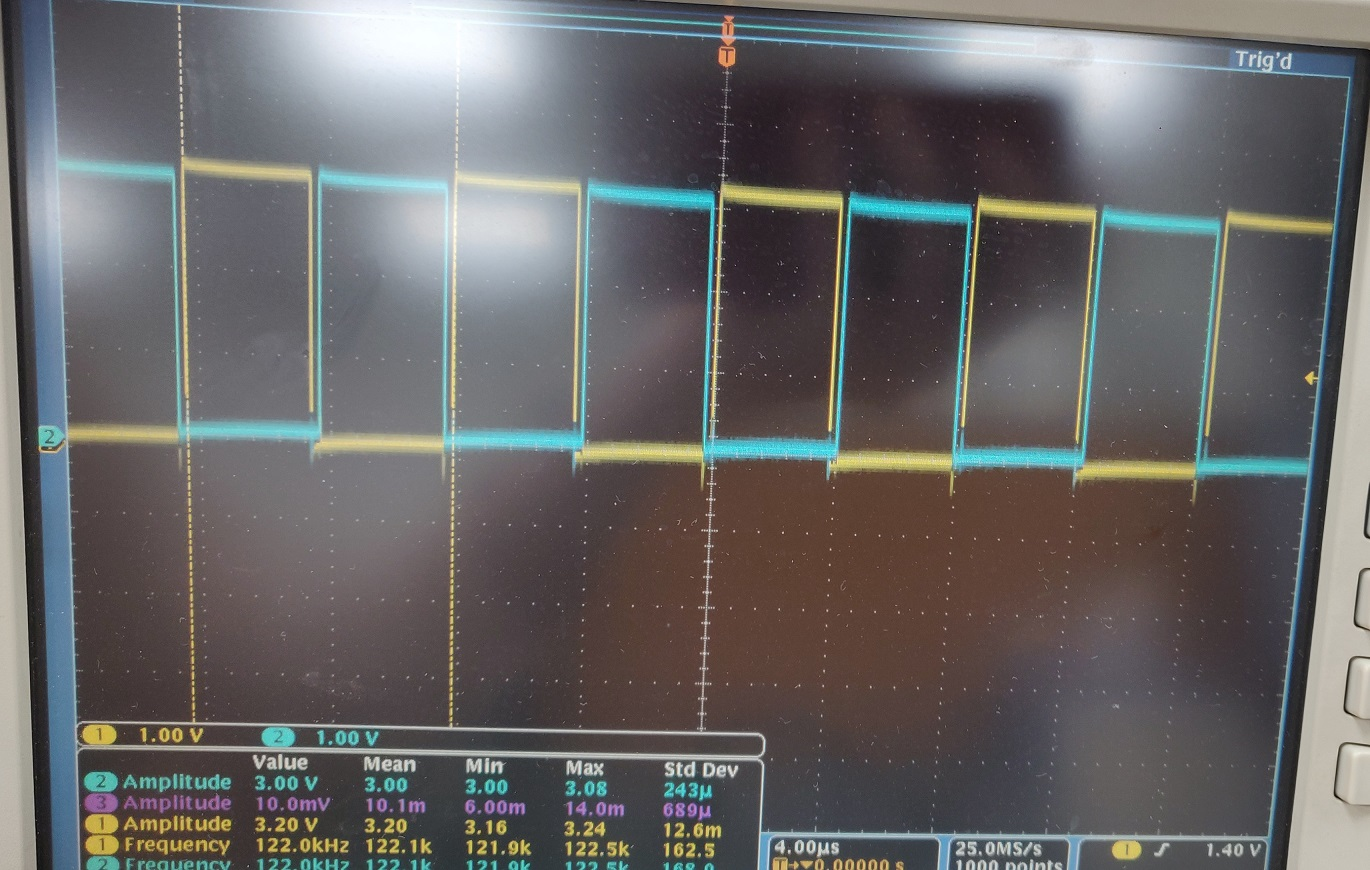
\includegraphics[width=.8\textwidth]{Figures/4_controlsystem_fpga_pwm.png}
	\caption{Complementary PWM output with Pynq Z1 FPGA and JupyterLab notebook}
	\label{fig:4_controlsystem_fpga_pwm}
\end{figure}
A preliminary implementation was implemented in Vivado and JupyterLab for a continuous complementary PWM controller. The resulting measurement can be seen in \cref{fig:4_controlsystem_fpga_pwm} before a clock configuration, which means the frequency corresponded to an arbitrary temporary pulse frequency of \qty{122}{\kilo\hertz}. As the initial test proved successful, the continued development and maturation of the pulser enabled a complete signal generator for the ultrasound pulse generator.

\begin{figure}[htbp]
	\centering
	\includegraphics[width=\linewidth]{Figures/5_controlsystem_fpga_pulser_logic.eps}
	\caption{Captured timing diagram of the control system pulser}
	\label{fig:5_controlsystem_pulser_logic}
\end{figure}
Seen in \cref{fig:5_controlsystem_pulser_logic} are the measured signals from the pulse generator showing the various timings of each signal captured with a Salae Logic Analyzer Pro 8.

\subsection{Power Stage}
Seen in \cref{fig:4_transmitter_meas} are actual measured inputs and outputs of the power stage. On the input, there are two complementary \qty{5}{\mega\hertz} signals with varying duty cycle to generate the desired dead time. On the output, we see the rail-to-rail push-pull operation of the \gls{mosfet} half-bridge. The schematic of the transmitter can be found in the appendix in \cref{fig:appendix_md1213db1}. Noticeable noise is observed in the input signal top and base but is negligible for successful operation. Possibly, the noise is due to a cable and adapter setup.
\begin{figure}[htbp]
	\centering
	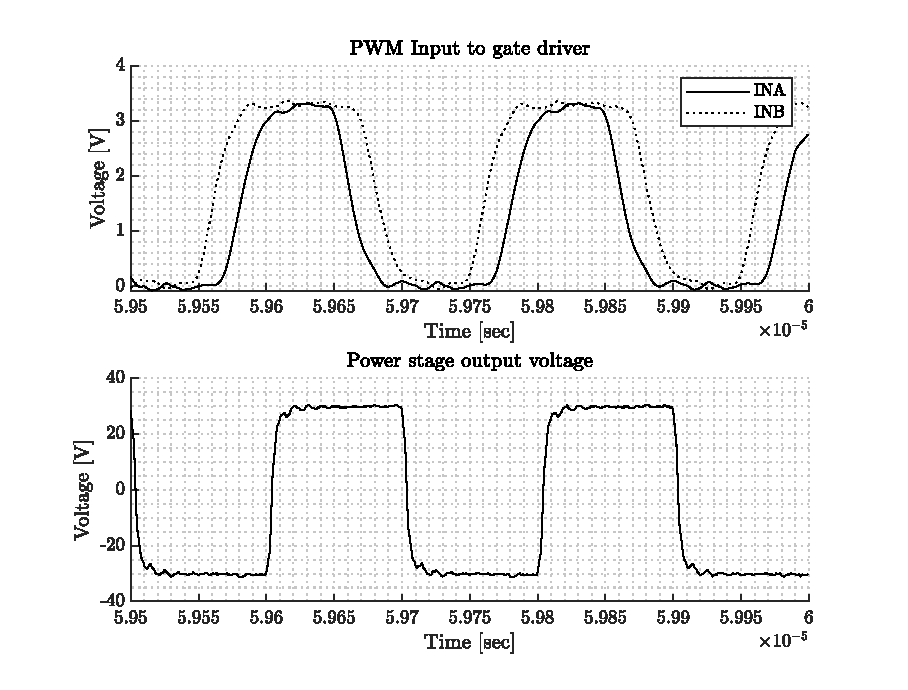
\includegraphics[width=.8\textwidth]{Figures/4_transmitter_pcb_out.eps}
	\caption[Measured input and output of power stage PCB]{Measured input and output of power stage PCB. (Above) Input to gate driver with dead-time (Below) Output of MOSFET half-bridge and the voltage across the load}
	\label{fig:4_transmitter_meas}
\end{figure}

\subsection{Transmit/Receive Switch}
\begin{figure}[htbp]
	\centering
	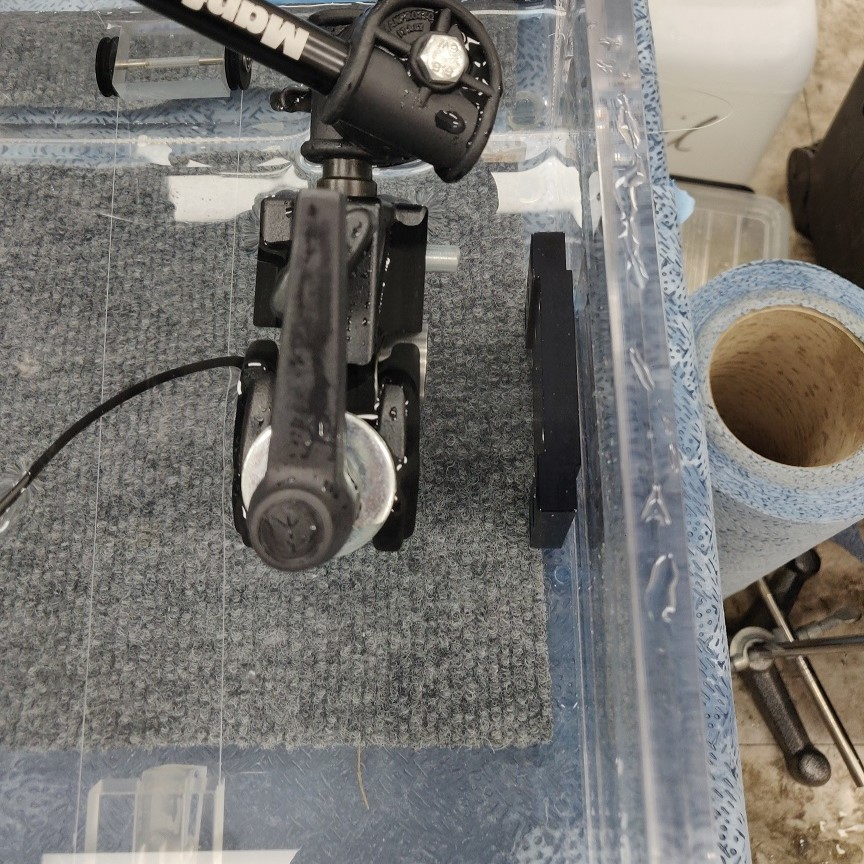
\includegraphics[width=.8\textwidth]{Figures/4_switch_meas_pic.jpg}
	\caption{TX/RX Switch reflection experiment with water tank}
	\label{fig:4_switch_meas_pic}
\end{figure}
For validating the TX/RX switch, an experiment is conducted with a \gls{pzt} transducer, water tank, function generator and an oscilloscope. Using two input signals, $f_{\mathrm{prf}}=\qty{10}{\kilo\hertz}$ switch signal, and $f_{0}=\qty{5}{\mega\hertz}$ burst mode transmit signal, the switch is configured to transmit and receive. A picture of the submerged transducer with a reflector can be seen in \cref{fig:4_switch_meas_pic}. After submerging the transducer in distilled water and measuring on the receiver side of the TX/RX switch, a reflected signal from the tank can be observed in \cref{fig:4_txrx_meas}.
\begin{figure}[htbp]
	\centering
	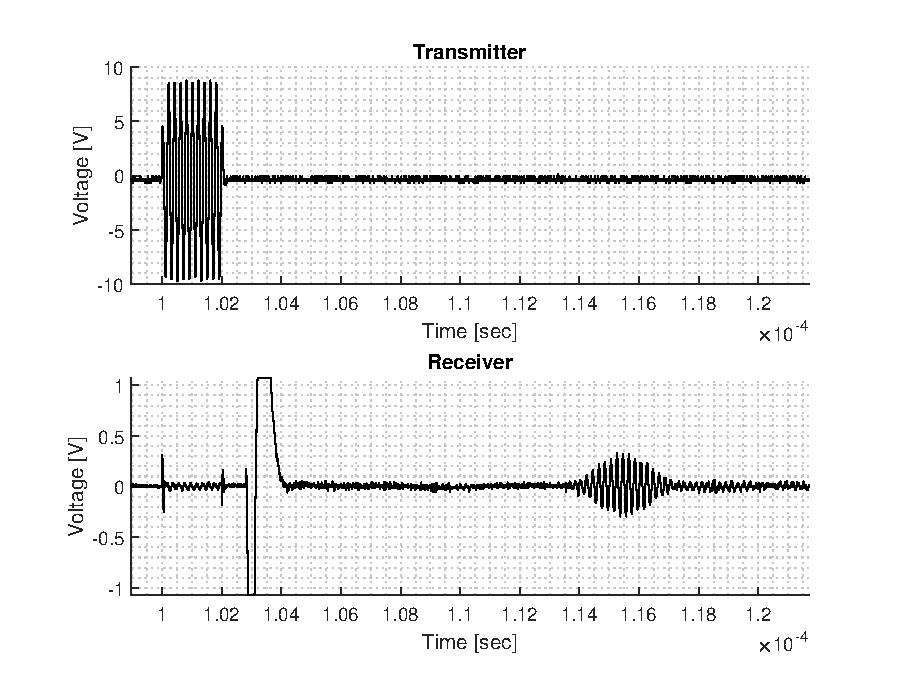
\includegraphics[width=.8\textwidth]{Figures/4_switch_pcb_meas.eps}
	\caption[Measured transmit and receive on Transmit/Receive Switch PCB]{Measured transmit and receive on Transmit/Receive Switch PCB (Above) Measured transmit voltage (Below) Received reflected signal off water tank}
	\label{fig:4_txrx_meas}
\end{figure}

\subsection{Band-pass Filter}
it is desired to validate its frequency response to determine if it functions as desired. To obtain the frequency response, a bode plot of the magnitude and phase is measured from \qty{300}{\kilo\hertz} until \qty{20}{\mega\hertz} using a \gls{vna} in a S21 configuration, meaning a measurement of the output in respect to the input. This measurement determines the difference in magnitude and phase of the output in comparison with the input signal. Observed in \cref{fig:4_bpf_measurement} is the frequency response of the band-pass filter measured on a \gls{vna}. It is noted that the pass band frequencies are mostly as expected with \qty{-0.5}{\decibel} frequencies at \qty{1.5}{\mega\hertz} and \qty{7}{\mega\hertz}. Though, the roll-off in the higher stop band appears somewhat lower than in the lower stop band. That would mean that it is plausible that higher frequency noise components are retained in the output than in the lower stop band. For the phase, it seems to have a significant phase delay, going from around \qty{100}{\degree} to \qty{250}{\degree} from the start to the end of the pass band.
\begin{figure}[htbp]
	\centering
	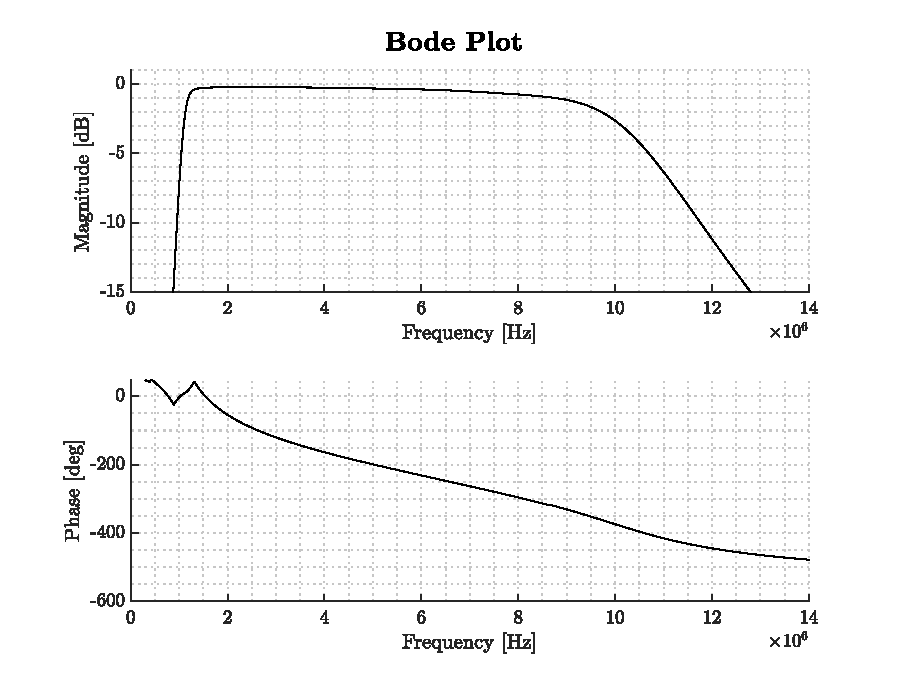
\includegraphics[width=.8\textwidth]{Figures/4_bpf_measurement_vna.eps}
	\caption[Band-pass filter bode plot]{Band-pass Filter bode plot from \qtyrange{0.3}{14}{\mega\hertz} with (above) magnitude and (below) phase}
	\label{fig:4_bpf_measurement}
\end{figure}

\subsection{Preamplifier}
Seen in \cref{fig:4_preamp_in} are measurements of the preamplifier circuits showing a \qty{70}{\milli\volt} input signal and a \qty{300}{\milli\volt} output signal with a \qty{2.5}{\volt} DC bias. In this application, however, only the \gls{lna} is used, and the \gls{vga} is bypassed in the hardware preamplifier configuration. The schematic of the preamplifier circuit is part of the demodulation schematic and can be found in the appendix in \cref{fig:appendix_ad8333}.
\begin{figure}[htbp]
	\centering
	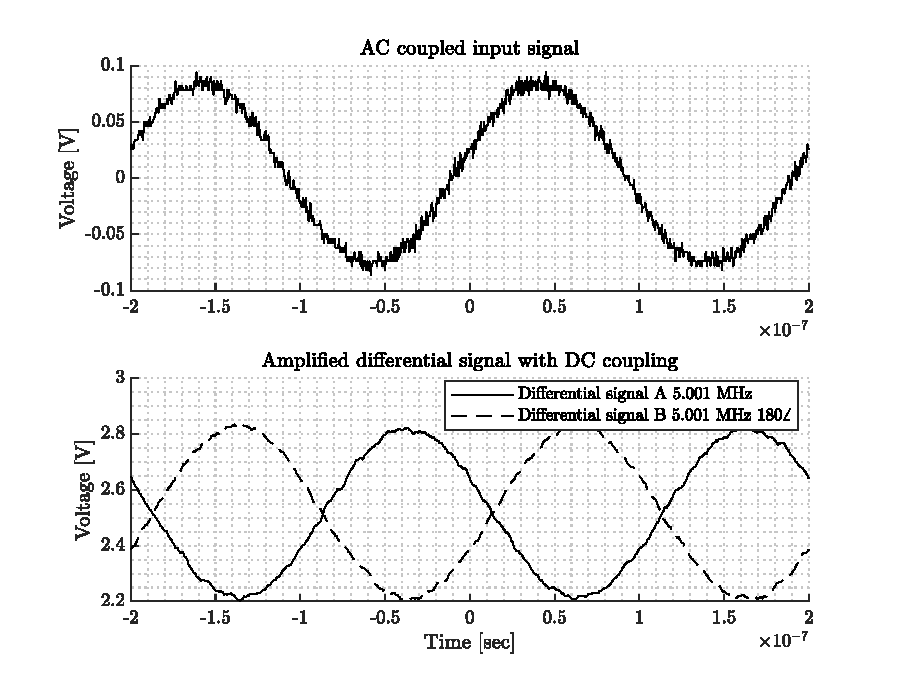
\includegraphics[width=.8\textwidth]{Figures/4_preamplifier_pcb.eps}
	\caption[Measured input and output of preamplifier PCB]{Measured input of preamplifier PCB, (Above) AC coupled input signal with amplitude \qty{1}{\volt} (Below Measured output of preamplifier PCB, Differential signal with DC coupling and $\times \qty{19}{\decibel}$ amplification)}
	\label{fig:4_preamp_in}
\end{figure}

\subsection{Demodulator}
An experiment is conducted with the sample-and-hold amplifier to verify the functionality. A low-frequency I-Q simulated signal is created from the function generator with a sample gating pulse train to control the sample-and-hold function. Seen in \cref{fig:4_demod_in} are the input signals, differential signals of \qty{5.001}{\mega\hertz} and \qty{20}{\mega\hertz} local oscillator signal. Seen in \cref{fig:4_demod_out} are the differential input signals $A$ and $B$ and the demodulated output signals $I$ and $Q$, where the phase between $I$ and $Q$ denotes the Doppler shift direction, or rather, the direction of flow of the scatterer. It is noted that the differential signal is so high frequency compared to the timescale so there has to be a zoomed in subplot where the waveform is visible to show the waveform. This highlights the observation of the Doppler shift being pushed down in frequency, which is one of the key functions of the demodulator in this system.

\begin{figure}[htbp]
	\centering
	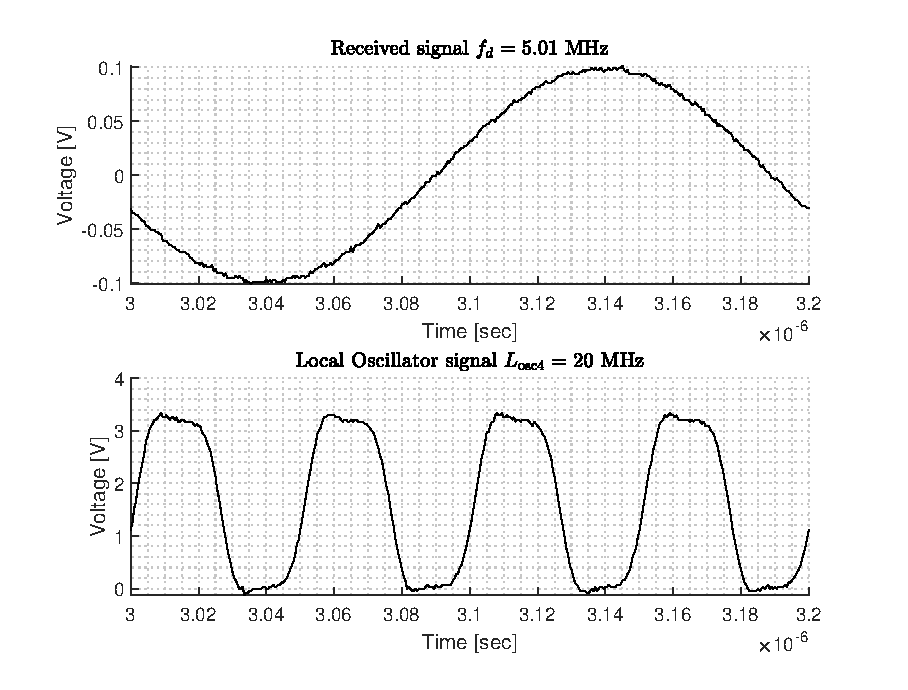
\includegraphics[width=.8\textwidth]{Figures/4_demod_pcb_in.eps}
	\caption[Measured input of demodulator PCB]{Measured input of demodulator PCB (Above) Input from received signal (Below) Input from local oscillator ($f_{0}\cdot4$)}
	\label{fig:4_demod_in}
\end{figure}
\begin{figure}[htbp]
	\centering
	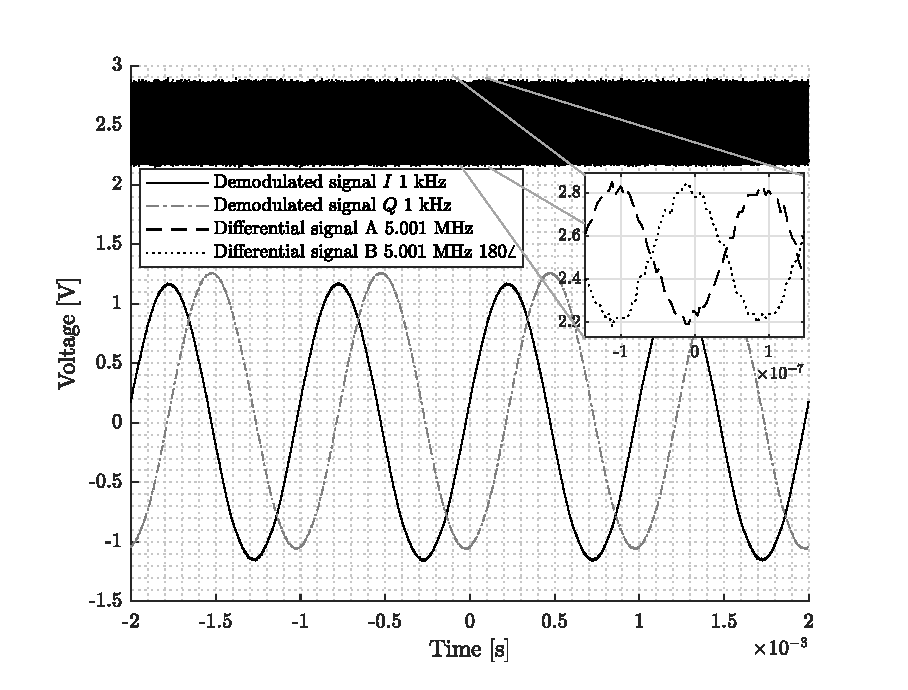
\includegraphics[width=.8\textwidth]{Figures/4_demod_pcb_out.eps}
	\caption[Measured output of demodulator PCB]{Measured output of demodulator PCB}
	\label{fig:4_demod_out}
\end{figure}

\subsection{Sample and Hold Amplifier}
Seen in \cref{fig:4_sample_hold_pcb} is the measured inputs and outputs of the circuit during the experiment. Above is the I-Q input and in the middle is the sample gating, and below is the output signal. On the output signal, it is noted the corresponding voltage transients for every pulse in the gate input.
\begin{figure}[htbp]
	\centering
	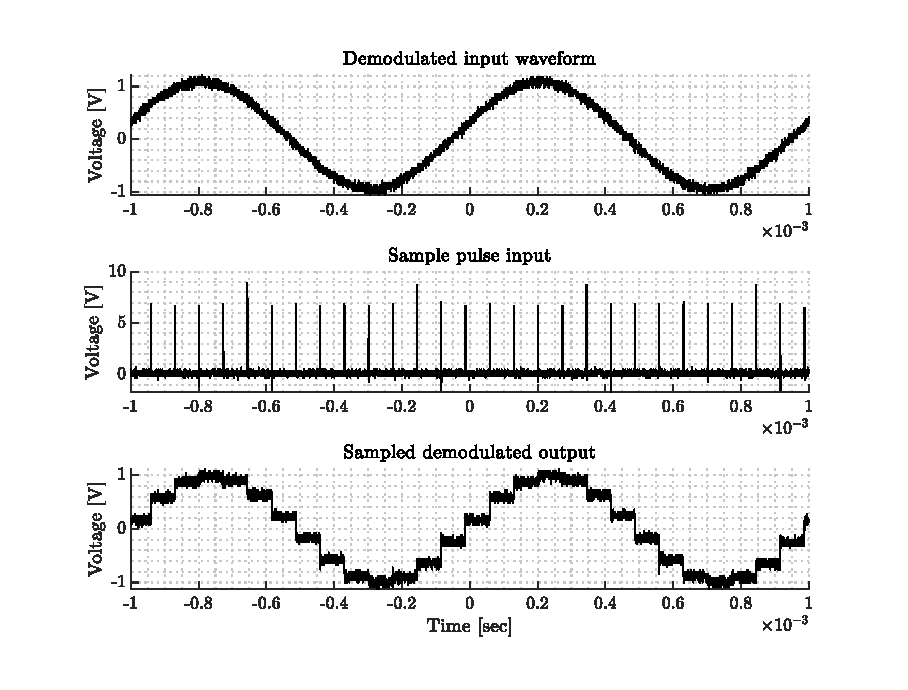
\includegraphics[width=.8\textwidth]{Figures/4_sampler_pcb.eps}
	\caption{Measured input and output of Sample and Hold amplifier}
	\label{fig:4_sample_hold_pcb}
\end{figure}

\subsection{Active Filter, DC Coupler}
\begin{figure}
	\centering
	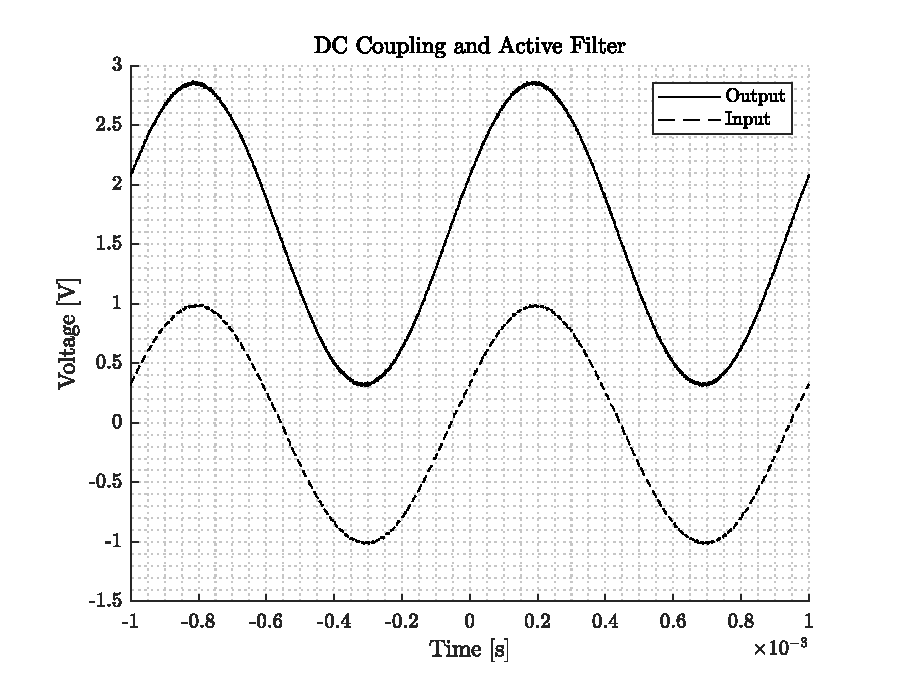
\includegraphics[width=.8\textwidth]{Figures/5_dccoupler_filter_measurement.eps}
	\caption{Measured input and output of Active filter and DC Coupler}
	\label{fig:5_dccoupler_measured}
\end{figure}
Seen in \cref{fig:5_dccoupler_measured} is the measured input and output of the DC coupler and active filter. The dashed line is the \gls{ac} coupled input signal with \qty{1}{\volt} amplitude and the solid line is the amplified \gls{dc} coupled output signal.

\section{Pulse Generator and Power Stage}
Using the pulse generator and the power stage, an experiment is performed where the complementary PWM signals are generated and output to the gate driver of the power stage. In turn, the gate driver will drive the MOSFET pair and output a high-power output than the pulse generator can supply on its own through its \gls{gpio}.

\begin{figure}[htbp]
	\centering
	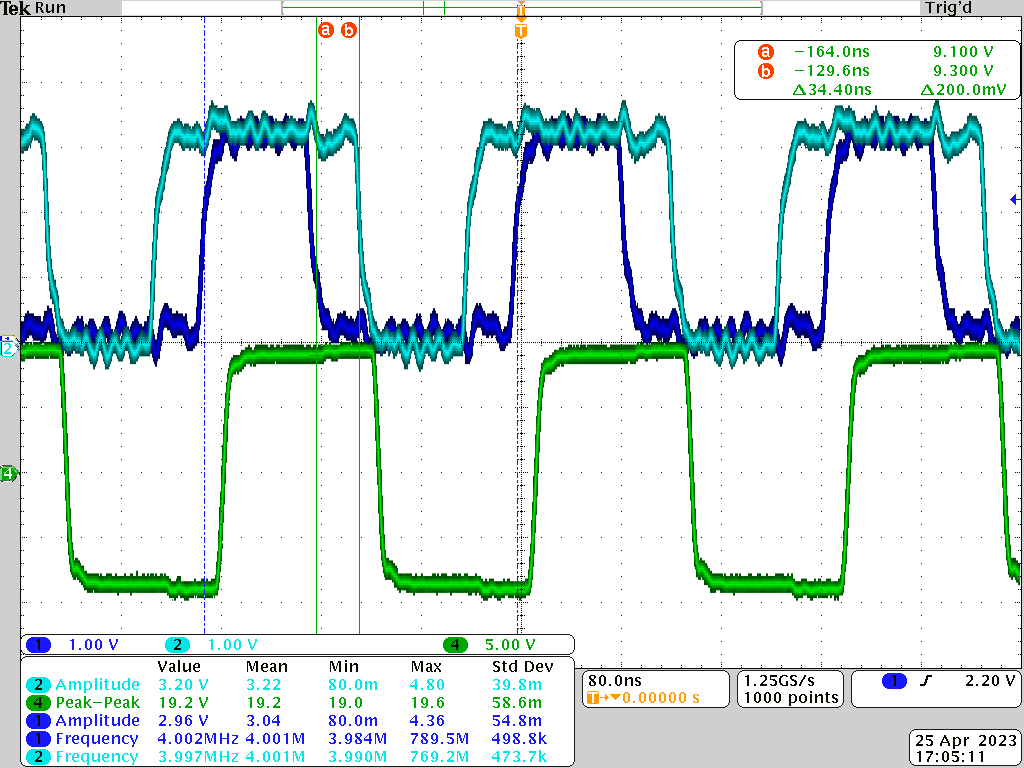
\includegraphics[width=.8\textwidth]{Figures/5_controlsystem_fpga_pwm.png}
	\caption{Complementary PWM output from the pulse generator and bipolar high power pulses}
	\label{fig:5_pulse_generator_experiment}
\end{figure}

Seen in \cref{fig:5_pulse_generator_experiment} are the measurements obtained from the pulse generator and power stage experiment. The measurements show the ability of the Pynq Z1 as a pulse generator is functioning as expected. As the power stage half-bridge is rail-to-rail, the output pulse voltages depend on the power supply voltage. In this case, the experiment is using a \qty{30}{\volt} maximum \gls{dcps}, and the output peak pulse voltages are $\pm \qty{30}{\volt}$. However, the power stage itself is specified for operating voltages up to $\pm \qty{100}{\volt}$.

\section{Doppler String Phantom Experiment}
The CIRS A043 Doppler String Phantom is a device used to evaluate the performance of Doppler ultrasound imaging systems. The phantom consists of a set of strings that move in a controlled manner when exposed to ultrasound waves. The strings are made of nylon monofilament and are arranged in a parallel array.

When the phantom is scanned with a Doppler ultrasound probe, the strings vibrate in response to the sound waves, producing a Doppler signal. The phantom includes a set of control strings that vibrate at a known frequency, allowing the user to calibrate the system and determine its accuracy. The string is driven by a motor that can be programmed to move at different speeds and directions, and it is also designed to create turbulence, which mimics the flow of blood in diseased vessels.

The phantom also includes a set of strings that move in a complex, non-linear pattern, simulating blood flow in vessels with turbulent flow. This allows the user to test the system's ability to accurately detect and measure turbulent blood flow, which is an important diagnostic feature for conditions such as stenosis or arterial occlusion.

By evaluating the system's performance on the known frequencies of the control strings and the complex patterns of the turbulence strings, the user can assess the accuracy and reliability of the Doppler ultrasound system. The CIRS A043 Doppler String Phantom is widely used in research, development, and quality assurance of Doppler ultrasound equipment.
\begin{figure}[htbp]
	\centering
	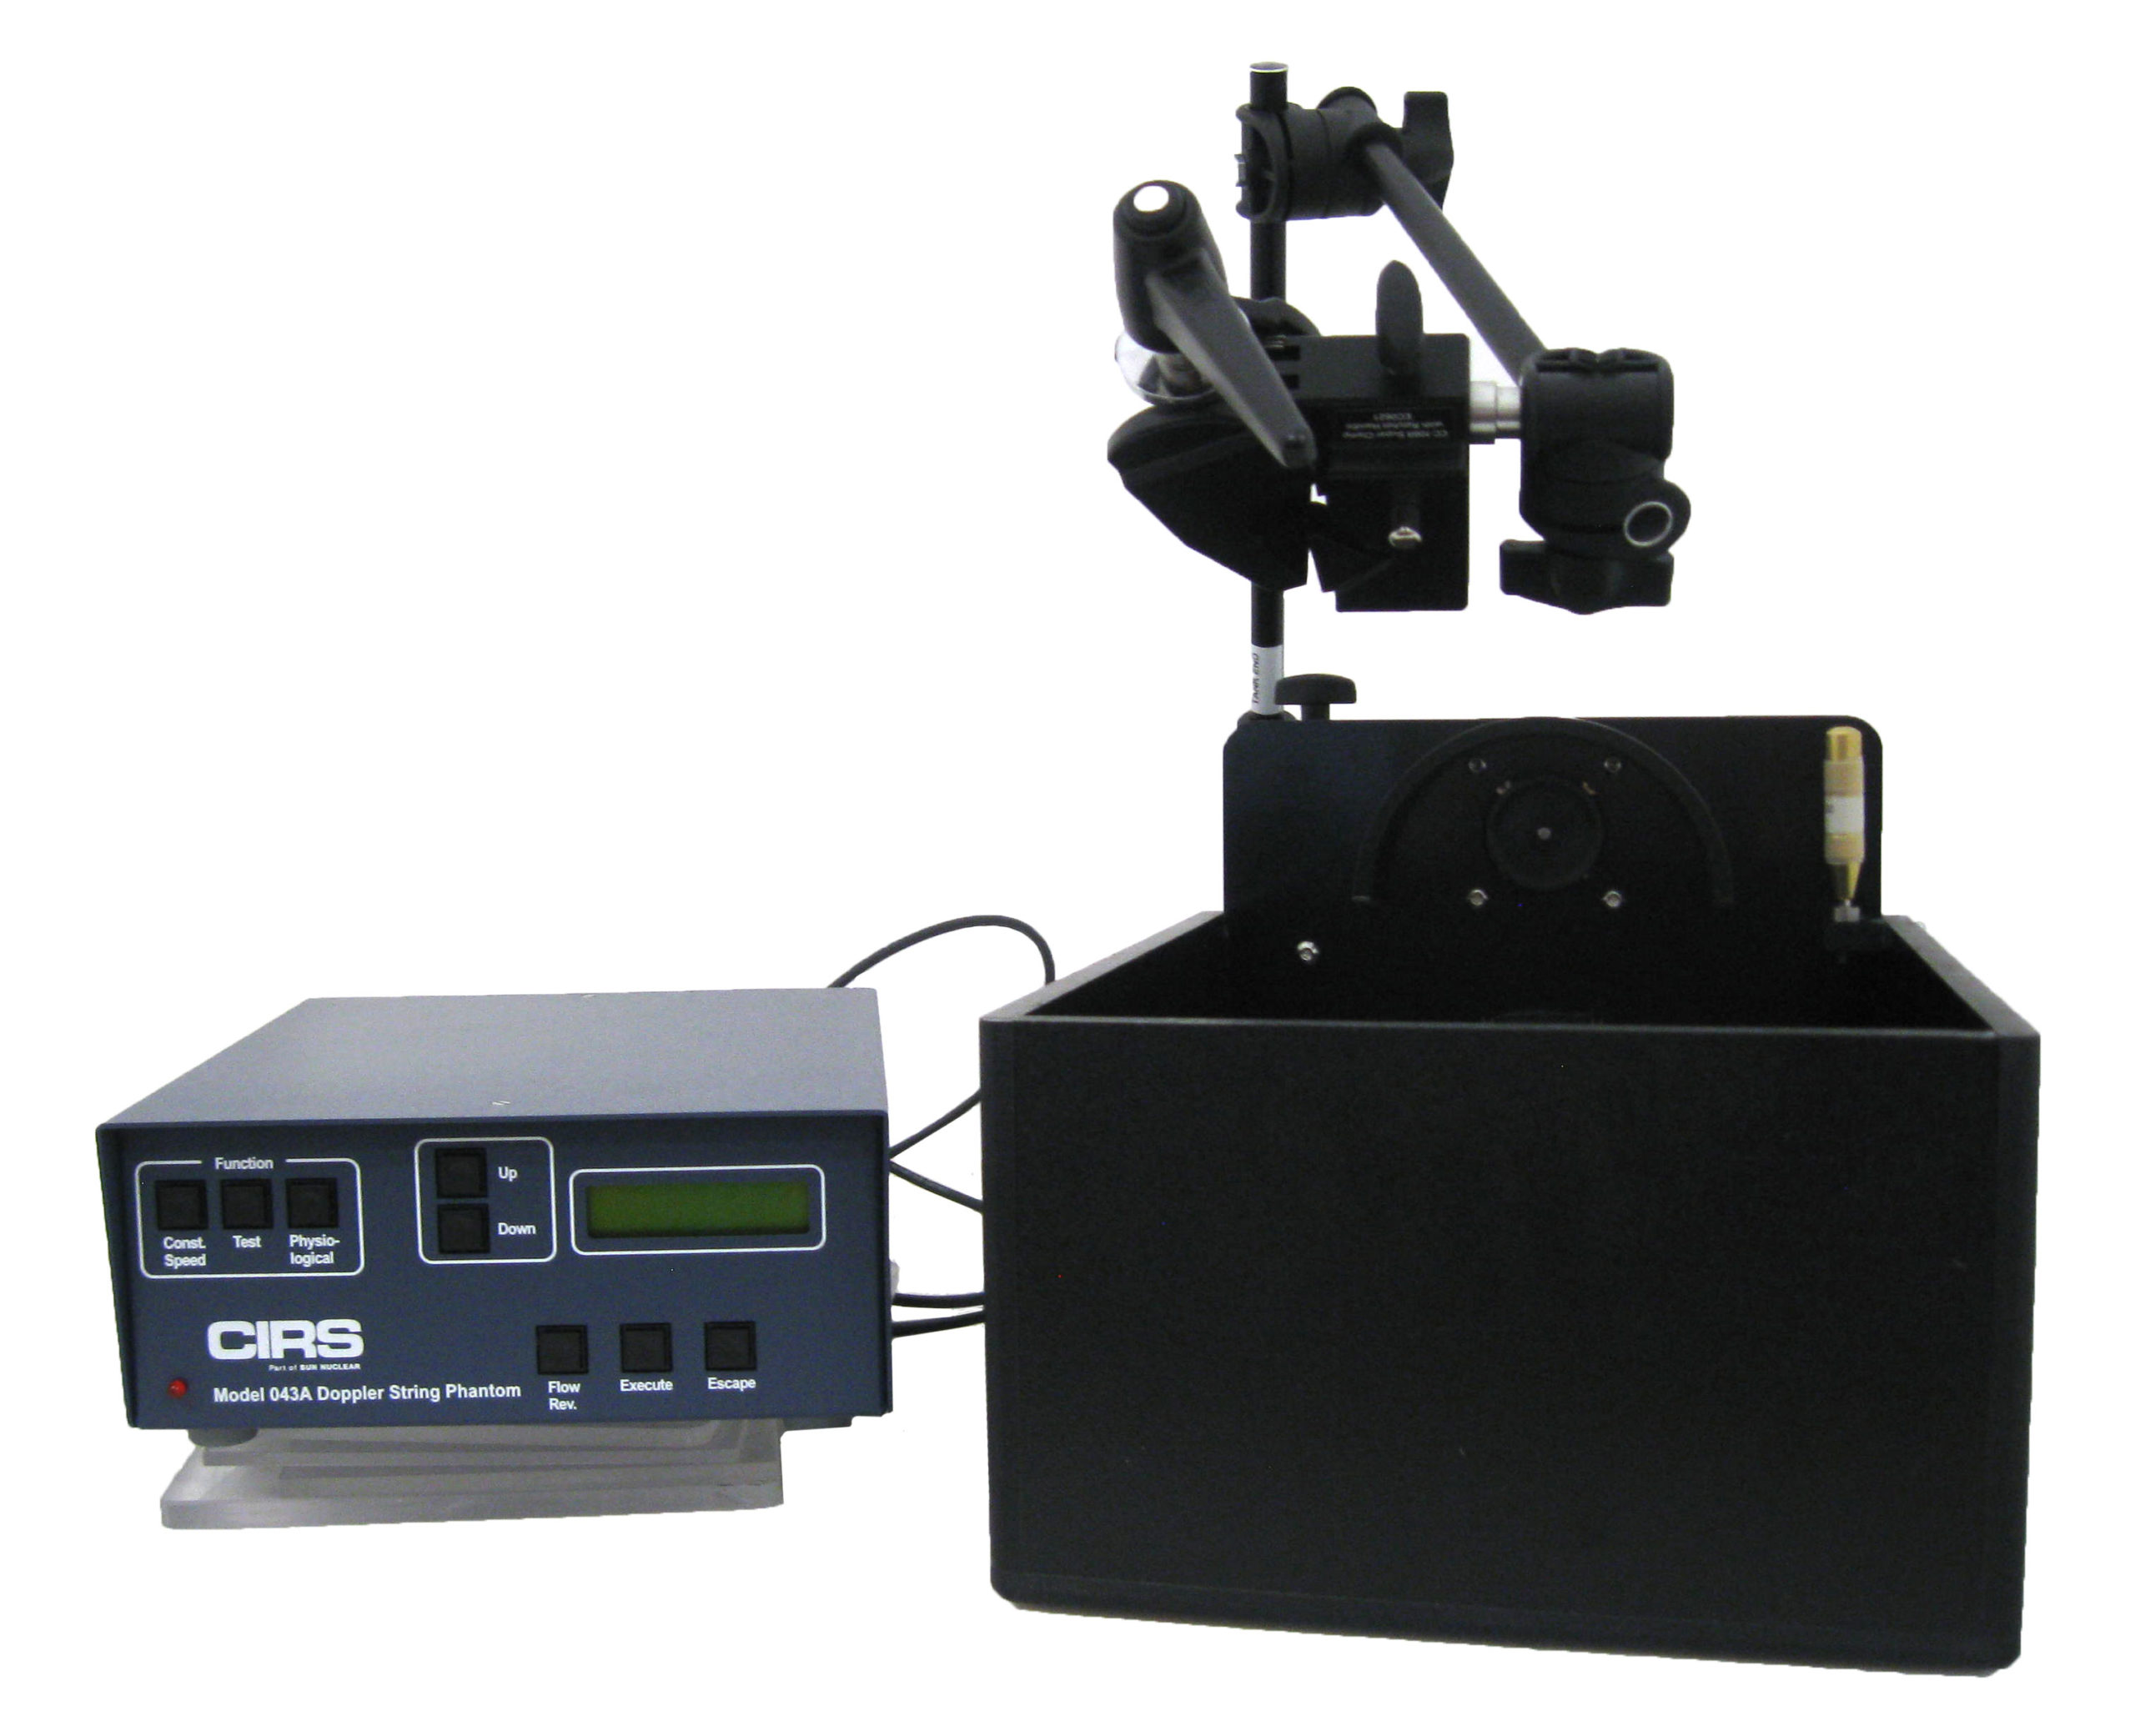
\includegraphics[width=.8\textwidth]{Figures/5_cirs_043a_image.jpg}
	\caption[CIRS Model 043A Doppler String Phantom]{CIRS Model 043A Doppler String Phantom with (left) motor controller and (right) tank and string loop}
\end{figure}

\begin{figure}[htbp]
	\centering
	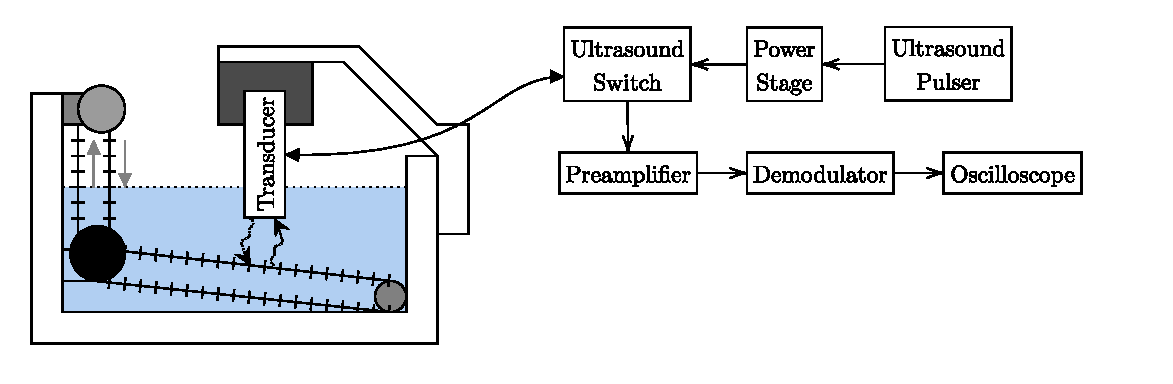
\includegraphics[width=.8\textwidth]{Figures/5_doppler_string_phantom_experiment.pdf}
	\caption{Doppler String Phantom experiment diagram (not to scale)}
	\label{fig:5_doppler_string_experiment}
\end{figure}
